\documentclass[12pt]{report}
\usepackage{scribe,graphicx,graphics}
\usepackage{proba}
\usepackage{float}
\usepackage{cancel}
\usepackage{listings}
\newcommand{\norm}[1]{\left|\left|#1\right|\right|}
\usepackage{listings}
\usepackage{xcolor}

\definecolor{codegreen}{rgb}{0,0.6,0}
\definecolor{codegray}{rgb}{0.5,0.5,0.5}
\definecolor{codepurple}{rgb}{0.58,0,0.82}
\definecolor{backcolour}{rgb}{0.95,0.95,0.92}

\lstdefinestyle{mystyle}{
    backgroundcolor=\color{backcolour},   
    commentstyle=\color{codegreen},
    keywordstyle=\color{magenta},
    numberstyle=\tiny\color{codegray},
    stringstyle=\color{codepurple},
    basicstyle=\ttfamily\footnotesize,
    breakatwhitespace=false,         
    breaklines=true,                 
    captionpos=b,                    
    keepspaces=true,                 
    numbers=left,                    
    numbersep=5pt,                  
    showspaces=false,                
    showstringspaces=false,
    showtabs=false,                  
    tabsize=2
}

\lstset{style=mystyle}
\course{CSE 382M} 	
\coursetitle{Found. Data Science \& ML}	
\semester{Spring 2025}
\lecturer{} % Due Date: {\bf Mon, Oct 3 2016}}
\lecturetitle{Problem Set}
\lecturenumber{1}   
\lecturedate{}    
\usepackage{enumerate}
\newcommand{\remind}[1]{\textcolor{red}{\textbf{#1}}} %To remind me of unfinished work to fix later
\newcommand{\hide}[1]{} %To hide large blocks of code without using % symbols

\newcommand{\ep}{\varepsilon}
\newcommand{\vp}{\varphi}
\newcommand{\lam}{\lambda}
\newcommand{\Lam}{\Lambda}
%\newcommand{\abs}[1]{\ensuremath{\left\lvert#1\right\rvert}} % This clashes with the physics package
%\newcommand{\norm}[1]{\ensuremath{\left\lVert#1\right\rVert}} % This clashes with the physics package
\newcommand{\floor}[1]{\ensuremath{\left\lfloor#1\right\rfloor}}
\newcommand{\ceil}[1]{\ensuremath{\left\lceil#1\right\rceil}}
\newcommand{\A}{\mathbb{A}}
\newcommand{\B}{\mathbb{B}}
\newcommand{\C}{\mathbb{C}}
\newcommand{\D}{\mathbb{D}}
\newcommand{\E}{\mathbb{E}}
\newcommand{\F}{\mathbb{F}}
\newcommand{\K}{\mathbb{K}}
\newcommand{\N}{\mathbb{N}}
\newcommand{\Q}{\mathbb{Q}}
\newcommand{\R}{\mathbb{R}}
\newcommand{\T}{\mathbb{T}}
\newcommand{\X}{\mathbb{X}}
\newcommand{\Y}{\mathbb{Y}}
\newcommand{\Z}{\mathbb{Z}}
\newcommand{\As}{\mathcal{A}}
\newcommand{\Bs}{\mathcal{B}}
\newcommand{\Cs}{\mathcal{C}}
\newcommand{\Ds}{\mathcal{D}}
\newcommand{\Es}{\mathcal{E}}
\newcommand{\Fs}{\mathcal{F}}
\newcommand{\Gs}{\mathcal{G}}
\newcommand{\Hs}{\mathcal{H}}
\newcommand{\Is}{\mathcal{I}}
\newcommand{\Js}{\mathcal{J}}
\newcommand{\Ks}{\mathcal{K}}
\newcommand{\Ls}{\mathcal{L}}
\newcommand{\Ms}{\mathcal{M}}
\newcommand{\Ns}{\mathcal{N}}
\newcommand{\Os}{\mathcal{O}}
\newcommand{\Ps}{\mathcal{P}}
\newcommand{\Qs}{\mathcal{Q}}
\newcommand{\Rs}{\mathcal{R}}
\newcommand{\Ss}{\mathcal{S}}
\newcommand{\Ts}{\mathcal{T}}
\newcommand{\Us}{\mathcal{U}}
\newcommand{\Vs}{\mathcal{V}}
\newcommand{\Ws}{\mathcal{W}}
\newcommand{\Xs}{\mathcal{X}}
\newcommand{\Ys}{\mathcal{Y}}
\newcommand{\Zs}{\mathcal{Z}}
\newcommand{\ab}{\textbf{a}}
\newcommand{\bb}{\textbf{b}}
\newcommand{\cb}{\textbf{c}}
\newcommand{\db}{\textbf{d}}
\newcommand{\ub}{\textbf{u}}
\newcommand{\sbb}{\textbf{s}}
%\renewcommand{\vb}{\textbf{v}} % This clashes with the physics package (the physics package already defines the \vb command)
\newcommand{\wb}{\textbf{w}}
\newcommand{\xb}{\textbf{x}}
\newcommand{\yb}{\textbf{y}}
\newcommand{\zb}{\textbf{z}}
\newcommand{\vbb}{\textbf{v}}
\newcommand{\Ab}{\textbf{A}}
\newcommand{\Bb}{\textbf{B}}
\newcommand{\Cb}{\textbf{C}}
\newcommand{\Db}{\textbf{D}}
\newcommand{\eb}{\textbf{e}}
\newcommand{\ex}{\textbf{e}_x}
\newcommand{\ey}{\textbf{e}_y}
\newcommand{\ez}{\textbf{e}_z}
\newcommand{\zerob}{\mathbf{0}}
\newcommand{\abar}{\overline{a}}
\newcommand{\bbar}{\overline{b}}
\newcommand{\cbar}{\overline{c}}
\newcommand{\dbar}{\overline{d}}
\newcommand{\ubar}{\overline{u}}
\newcommand{\vbar}{\overline{v}}
\newcommand{\wbar}{\overline{w}}
\newcommand{\xbar}{\overline{x}}
\newcommand{\ybar}{\overline{y}}
\newcommand{\zbar}{\overline{z}}
\newcommand{\Abar}{\overline{A}}
\newcommand{\Bbar}{\overline{B}}
\newcommand{\Cbar}{\overline{C}}
\newcommand{\Dbar}{\overline{D}}
\newcommand{\Ubar}{\overline{U}}
\newcommand{\Vbar}{\overline{V}}
\newcommand{\Wbar}{\overline{W}}
\newcommand{\Xbar}{\overline{X}}
\newcommand{\Ybar}{\overline{Y}}
\newcommand{\Zbar}{\overline{Z}}
\newcommand{\Aint}{A^\circ}
\newcommand{\Bint}{B^\circ}
\newcommand{\limk}{\lim_{k\to\infty}}
\newcommand{\limm}{\lim_{m\to\infty}}
\newcommand{\limn}{\lim_{n\to\infty}}
\newcommand{\limx}[1][a]{\lim_{x\to#1}}
\newcommand{\liminfm}{\liminf_{m\to\infty}}
\newcommand{\limsupm}{\limsup_{m\to\infty}}
\newcommand{\liminfn}{\liminf_{n\to\infty}}
\newcommand{\limsupn}{\limsup_{n\to\infty}}
\newcommand{\sumkn}{\sum_{k=1}^n}
\newcommand{\sumk}[1][1]{\sum_{k=#1}^\infty}
\newcommand{\summ}[1][1]{\sum_{m=#1}^\infty}
\newcommand{\sumn}[1][1]{\sum_{n=#1}^\infty}
\newcommand{\emp}{\varnothing}
\newcommand{\exc}{\backslash}
\newcommand{\sub}{\subseteq}
\newcommand{\sups}{\supseteq}
\newcommand{\capp}{\bigcap}
\newcommand{\cupp}{\bigcup}
\newcommand{\kupp}{\bigsqcup}
\newcommand{\cappkn}{\bigcap_{k=1}^n}
\newcommand{\cuppkn}{\bigcup_{k=1}^n}
\newcommand{\kuppkn}{\bigsqcup_{k=1}^n}
\newcommand{\cappk}[1][1]{\bigcap_{k=#1}^\infty}
\newcommand{\cuppk}[1][1]{\bigcup_{k=#1}^\infty}
\newcommand{\cappm}[1][1]{\bigcap_{m=#1}^\infty}
\newcommand{\cuppm}[1][1]{\bigcup_{m=#1}^\infty}
\newcommand{\cappn}[1][1]{\bigcap_{n=#1}^\infty}
\newcommand{\cuppn}[1][1]{\bigcup_{n=#1}^\infty}
\newcommand{\kuppk}[1][1]{\bigsqcup_{k=#1}^\infty}
\newcommand{\kuppm}[1][1]{\bigsqcup_{m=#1}^\infty}
\newcommand{\kuppn}[1][1]{\bigsqcup_{n=#1}^\infty}
\newcommand{\cappa}{\bigcap_{\alpha\in I}}
\newcommand{\cuppa}{\bigcup_{\alpha\in I}}
\newcommand{\kuppa}{\bigsqcup_{\alpha\in I}}
\newcommand{\Rx}{\overline{\mathbb{R}}}
\newcommand{\dx}{\,dx}
\newcommand{\dy}{\,dy}
\newcommand{\dt}{\,dt}
\newcommand{\dax}{\,d\alpha(x)}
\newcommand{\dbx}{\,d\beta(x)}
\DeclareMathOperator{\glb}{\text{glb}}
\DeclareMathOperator{\lub}{\text{lub}}
\newcommand{\xh}{\widehat{x}}
\newcommand{\yh}{\widehat{y}}
\newcommand{\zh}{\widehat{z}}
\newcommand{\<}{\langle}
\renewcommand{\>}{\rangle}
\renewcommand{\iff}{\Leftrightarrow}
\DeclareMathOperator{\im}{\text{im}}
\let\spn\relax\let\Re\relax\let\Im\relax
\DeclareMathOperator{\spn}{\text{span}}
\DeclareMathOperator{\sym}{\text{Sym}}
\DeclareMathOperator{\myskew}{\text{Skew}}
\DeclareMathOperator{\Re}{\text{Re}}
\DeclareMathOperator{\Im}{\text{Im}}
\DeclareMathOperator{\diag}{\text{diag}}
\endinput

% Insert your name here!
\scribe{Student Name: Noah Reef}

\begin{document}
\maketitle
\section*{Problem 1}
Let $x \in \R^d \sim \mathcal{N}(0,I_d)$ and $e_1$ be the canonical vector with $1$ in the first coordinate and $0$ otherwise. Then we see that
\begin{equation*}
    x \cdot e_1 = x_1 \sim \mathcal{N}(0,1)
\end{equation*}
if $v$ is an arbitrary non-zero vector in $\R^d$ then we have that
\begin{equation*}
    x \cdot v = \sum_{i=1}^d x_iv_i
\end{equation*}
where each $x_iv_i \sim \mathcal{N}(0,v_i^2)$, since
\begin{equation*}
    \VarX{v_i \cdot x_i} = v_i^2 \VarX{x_i} = v_i^2
\end{equation*}
and hence
\begin{equation*}
x \cdot v \sim \mathcal{N}\left(0,\sum_{i=1}^d v_i^2\right) = \mathcal{N}(0, \norm{v}_2^2)
\end{equation*}

\section*{Problem 2}
Below are the plots of frequency of distances between points normally sampled on the unit spheres in $\R^3$ and $\R^{100}$, respectively.
\begin{figure}[H]
    \centering
    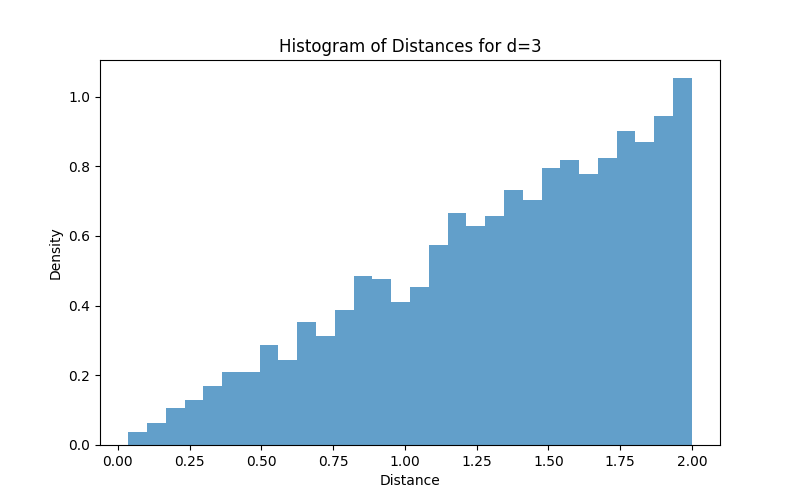
\includegraphics[scale=0.6]{CSE_382M/ps_1/dist_d_3.png}
    \caption{Case of $d = 3$}
    \label{fig:enter-label}
\end{figure}
\begin{figure}[H]
    \centering
    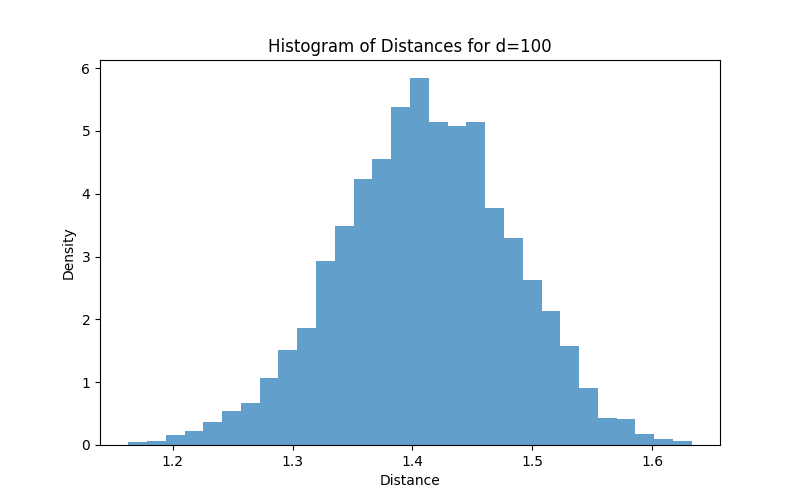
\includegraphics[scale=0.6]{CSE_382M/ps_1/dist_d_100.png}
    \caption{Case of $d=100$}
    \label{fig:enter-label}
\end{figure}
Here we see that in case that $d = 3$, the frequency of distances scales linearly while in the case of $d =100$ the frequency of distances follows a normal distribution as expected.

\section*{Problem 3}
Let $x \in \R^d$ with $\norm{x}_2 = 1$. Let $u = (1/\sqrt{k})Rx$ where $u \in \R^k$ and

\begin{equation*}
    R_{ij} = \begin{cases}
        \phantom{-}1 & p = 0.5 \\
        -1 & p = 0.5
    \end{cases}
\end{equation*}
\subsection*{Part a}
\begin{align*}
    \EX{\norm{u}_2^2} &= \EX{\sum_{i=1}^k\left(\sum_{j=1}^d \frac{1}{\sqrt{k}} R_{ij} x_j\right)^2} \\
    &= \frac{1}{k} \sum_{i=1}^k \EX{\left(\sum_{j=1}^d  R_{ij} x_j\right)^2} \\
    &= \frac{1}{k} \sum_{i=1}^k \EX{\sum_{j=1}^d  \cancelto{1}{R_{ij}^2} x_j^2 + \sum_{j\neq j'} R_{ij}R_{ij'}x_jx_{j'}} \\
    &= \frac{1}{k}\sum_{i=1}^k \left(\EX{\norm{x}_2^2} + \sum_{j\neq j'}\cancelto{0}{\EX{R_{ij}R_{ij'}}}\EX{x_jx_{j'}} \right) \\
    &= \frac{1}{k} \sum_{i=1}^k 1 \\
    &= 1
\end{align*}
and
\begin{align*}
    \VarX{\norm{u}_2^2} &= \EX{(\norm{u}_2^2 - \EX{\norm{u}_2^2})^2} \\
    &= \EX{(\norm{u}_2^2 - 1)^2} \\
    &= \EX{\norm{u}_2^4}- 2\EX{\norm{u}_2^2} + 1 \\
    &= \EX{\norm{u}_2^4} - 1
\end{align*}
with
\begin{align*}
    \EX{\norm{u}_2^4} &= \frac{1}{k^2}\EX{\sum_{i=1}^k\left(\sum_{j=1}^dR_{ij}x_j\right)^4 + \sum_{i \neq i'}^k \left(\sum_{j=1}^dR_{ij}x_j\right)^2 \left(\sum_{j=1}^dR_{i'j}x_j\right)^2} \\
    &= \frac{1}{k}\left(3 - 2\sum_{j=1}^dx_j^4\right) + 1 - \frac{1}{k} = 1 + \frac{2}{k}\left(1 - \sum_{j=1}^d x_j^4\right) \leq 1 + \frac{2}{k}
\end{align*}
thus 
\begin{equation*}
     \VarX{\norm{u}_2^2} = \EX{\norm{u}_2^4} - 1 \leq \frac{2}{k}
\end{equation*}

\subsection*{Part b}
Suppose we want the following probability 
\begin{equation*}
    \Pr[\norm{u}_2^2 - 1 \leq \epsilon] = 1 - \Pr[\norm{u}_2^2 - 1 \geq \epsilon] = 1-\delta
\end{equation*}
then we have that by Chebyshev's inequality that
\begin{equation*}
    \Pr[\norm{u}_2^2 - 1 \geq \epsilon] = \delta \leq \frac{\VarX{\norm{u}_2^2}}{\epsilon^2} = \frac{2}{k\epsilon^2}
\end{equation*}
re-arranging terms for $k$ we get that
\begin{equation*}
    k \geq \frac{2}{\delta \epsilon^2}
\end{equation*}
\subsection*{Part c}
\begin{figure}[H]
    \centering
    \begin{lstlisting}[language=python]
import numpy as np

d = 1000
delta = 1/3
epsilon = 0.1

# Choose k_max using the Gaussian sharper bound
k_max = 2/(delta * epsilon**2)
#k_max = 2/(epsilon**2) * np.log(1/delta)
k = int(min(k_max, d/2))

def random_sign_projection(x, k):
    d = len(x)
    R = np.random.choice([-1, 1], size=(k, d))
    u = (1/np.sqrt(k)) * R @ x
    return np.linalg.norm(u)**2

def gaussian_projection(x, k):
    d = len(x)
    G = np.random.randn(k, d) / np.sqrt(k)
    u = G @ x
    return np.linalg.norm(u)**2

num_trials = 1000
R_violate_terms = 0
G_violate_terms = 0

for trial in range(num_trials):
    # Generate a random unit vector in R^d
    x = np.random.randn(d)
    x = x / np.linalg.norm(x)  # Normalize x
    
    u_R = random_sign_projection(x, k)
    u_G = gaussian_projection(x, k)

    # Check both sides of the deviation: |u - 1| > epsilon
    if abs(u_R - 1) > epsilon:
        R_violate_terms += 1
    if abs(u_G - 1) > epsilon:
        G_violate_terms += 1

print(R_violate_terms / num_trials)
print(G_violate_terms / num_trials)
    \end{lstlisting}
    \caption{Numerical Experiment for bounds of $R$ and $G$}
    \label{fig:enter-label}
\end{figure}

and see that

\begin{table}[H]
    \centering
    \begin{tabular}{c|c|c}
         & $\delta_R$  & $\delta_G$  \\ 
        \hline $\frac{2}{\delta \epsilon^2}$ &$0.104$  & $0.1$\\ 
        \hline $\frac{2}{\epsilon^2} \ln(1/\delta)$& $0.297$  & $0.291$ \\
    \end{tabular}
    \caption{Numerical Estimates for $\delta$ with different bounds}
    \label{tab:my_label}
\end{table}
Thus we see that $G$ violates the inequality with higher probability than $R$, and hence is more accurate. 
\section*{Problem 4}
\subsection*{Part a}
\begin{equation*}
    (HD)^*(HD) = D^*H^*HD
\end{equation*}
see that for $d = 1$
\begin{equation*}
    H_1^*H_1 = \frac{1}{2} \begin{bmatrix}
        1 & 1 \\
        1 & -1
    \end{bmatrix}\begin{bmatrix}
        1 & 1 \\
        1 & -1
    \end{bmatrix} = \frac{1}{2}\begin{bmatrix}
        2 & 0 \\
        0 & 2
    \end{bmatrix} = I_2
\end{equation*}
then suppose that above holds for $d = k$ then we see for $d = k + 1$ that
\begin{equation*}
    H_{k+1} = \frac{1}{\sqrt{2}}\begin{bmatrix}
        H_k & H_k \\
        H_k & -H_k
    \end{bmatrix}
\end{equation*}
and thus
\begin{equation*}
    H_{k+1}^*H_{k+1} = \frac{1}{2}\begin{bmatrix}
        H_k^*H_k + H_k^*H_k & 0 \\
        0 & H_k^*H_k + H_k^*H_k
    \end{bmatrix} =\frac{1}{2} \begin{bmatrix}
        2I_k & 0 \\
        0 & 2I_k
    \end{bmatrix} = I_{k+1}
\end{equation*}
hence we have that
\begin{equation*}
     D^*H^*HD = D^*D = D^2 = I
\end{equation*}
thus $HD$ is a unitary matrix.
\subsection*{Part b}
Let $u = HDx$, then we have that
\begin{equation*}
    u_i = (HDx)_i = \sum_{j=1}^d H_{ij}D_{jj} x_j
\end{equation*}
note that each $H_{ij}D_{ji}x_j$ is random variable, since $D_{jj}$ is a random variable, such that
\begin{equation*}
    -H_{ij}x_j \leq H_{ij}D_{jj}x_j \leq H_{ij}x_j
\end{equation*}
and $|H_{ij}x_j| = (1/\sqrt{2})x_j$. Additionally we can compute
\begin{equation*}
    \Pr[|u_i| \geq \epsilon \norm{x}_2] = \Pr\left[\left|\sum_{j=1}^d H_{ij}D_{jj} x_j\right| \geq \epsilon \norm{x}_2\right] \leq 2\exp\left(-\frac{d\epsilon^2}{2}\right)
\end{equation*}
applying a union bound over all $i$ yields
\begin{equation*}
    \Pr[\max_i |u_i| \geq \epsilon \norm{x}_2] \leq 2d\exp\left(-\frac{d\epsilon^2}{2}\right) \leq \delta 
\end{equation*}
solving for $\epsilon$ we get
\begin{equation*}
    \epsilon = \sqrt{\frac{2 \ln(2d/\delta)}{d}}
\end{equation*}
and hence with probability of at least $1-\delta$ we have
\begin{equation*}
    \norm{u}_\infty = \norm{HDx}_\infty \leq \epsilon \norm{x}_2 = \sqrt{\frac{2 \ln(2d/\delta)}{d}} \norm{u}_2
\end{equation*}

\subsection*{Part c}
Let $n$ denote the number of non-zero entries, then from above we have
\begin{equation*}
    \norm{u}_2^2 \leq n \cdot \left( \sqrt{\frac{2 \ln(2d/\delta)}{d}} \norm{u}_2\right)^2
\end{equation*}
then solving for $n$ yields
\begin{equation*}
    n \geq \frac{d}{2\ln(2d/\delta)}
\end{equation*}
therefore the number of zero entries is at most
\begin{equation*}
    d -  \frac{d}{2\ln(2d/\delta)}
\end{equation*}
\section*{Problem 5}
\begin{figure}[H]
    \centering
\begin{lstlisting}[language=python]
import numpy as np

def algorithm_1(d,k):
  A = np.random.randn(d,d)
  A = A[0:k,:]

  return A

def algorithm_2(d,k):
  A = np.random.randn(k,d)
  return A

def compute_err(A):
  num_rows, num_cols = A.shape
  total_err = 0
  for i in range(num_cols):
    for j in range(i+1, num_cols):
      total_err += abs(np.dot(A[:,i],A[:,j]))
  return total_err



d = 1000
k = 800

algorithm_1_avg_err = 0
algorithm_2_avg_err = 0

for i in range(10):

  A = algorithm_1(d,k)
  err = compute_err(A)
  algorithm_1_avg_err += err

  A = algorithm_2(d,k)
  err = compute_err(A)
  algorithm_2_avg_err += err

algorithm_1_avg_err /= 10
algorithm_2_avg_err /= 10

print(algorithm_1_avg_err)
print(algorithm_2_avg_err)
\end{lstlisting}
\caption{Problem 5 Code for $k = 800$}
    \label{fig:enter-label}
\end{figure}
We can see that \texttt{algorithm\_1} will be more accurate (which agrees with experiment) since each vector is initially in $\R^d$ with $d > k$ and hence when sampled via a Gaussian we have that they are more likely to be orthogonal, however it will be slower than \texttt{algorithm\_2} since we compute extra $(d-k)$ terms for each sampled vector.
\end{document}